\documentclass[12pt]{article}
% Some custom commands to make typing easier. Feel free to add to it


% quick homomorphism
\newcommand{\homo}[1]{\varphi (#1)}
% quick inverse
\newcommand{\inv}[1]{#1^{-1}}
% quick generating set
\newcommand{\genset}[1]{\langle #1 \rangle}
% split problem into multiple parts
\newcommand{\spl}{\rule{\textwidth}{0.4pt}}
% quick normal subgroup
\newcommand{\nsub}{\trianglelefteq}
% quick Z/nZ
\newcommand{\znz}[1]{\mathbb{Z\text{/#1}Z}}
% quick stirling numbers
% \newcommand{\squig}{\genfrac{\lbrace}{\rbrace}{0pt}{}}
\newcommand{\squig}[2]{\left\{{#1 \atop #2}\right\}}


% quick projective surface
\newcommand{\proj}[1]{\mathbb P^{#1}(\mathbb C)}
% quick elliptic curve
\newcommand{\ellip}{E(\mathbb{C})}
% quick ramification
\newcommand{\ram}[1]{e_{#1}}

% todo list
\usepackage[color=yellow]{todonotes}
\newcommand{\tbd}[1]{\todo[inline]{#1}
\addcontentsline{toc}{subsubsection}{TODO}}

% scaling tikz
\usepackage{adjustbox}

% format bullets
% \usepackage[shortlabels]{enumitem}

% Document inherent packages to be loaded
\usepackage{amsmath, amsfonts, amssymb, amsthm, graphicx, url, xcolor, enumerate, tcolorbox}

%geometry helps manage margins, among other things.
\usepackage[rmargin=2in,lmargin=1in,tmargin=1in,bmargin=1in]{geometry}
\newcommand{\sidenote}[1]{\marginpar{\footnotesize \begin{itemize}
    \item[$\leftarrow$]\raggedright #1
\end{itemize}}}

\setlength{\headheight}{16pt}
\setlength{\marginparwidth}{1.5in}
\makeatletter      % make title smaller   
\def\@maketitle{   % custom maketitle 
\begin{center}
    {\Large \@title} \\[0.1in] \@author \\ {\small \@date}
\end{center}  
}
\setcounter{secnumdepth}{0}

% new color for the hypers
\definecolor{hyperpurp}{RGB}{108,113,196}
\usepackage[colorlinks = true,
            linkcolor = hyperpurp,
            urlcolor  = hyperpurp,
            citecolor = hyperpurp,
            anchorcolor = hyperpurp]{hyperref}

\usepackage[all,2cell,ps]{xy}
\usepackage{tikz, tikz-cd}
\usepackage{faktor}
\allowdisplaybreaks
\graphicspath{{Images/}}

\theoremstyle{definition}  % to get rid of the italics
\newtheorem{theorem}{\bt{Theorem}}%[section]
\newtheorem{proposition}[theorem]{\bt{Proposition}}
\newtheorem{corollary}[theorem]{\gt{Corollary}}
\newtheorem{lemma}[theorem]{\bt{Lemma}}
\newtheorem{conjecture}[theorem]{Conjecture}

\newtheorem{defn}{\rt{Definition}}

\newtheorem{eg}{\textcolor{violet}{Example}}
\newtheorem{cautiouseg}[eg]{\textcolor{magenta}{Tricky example}}
\newtheorem{noneg}[eg]{\textcolor{violet}{Non-example}}

\newtheorem*{rmk}{Remark}


%Import the natbib package and sets a bibliography  and citation styles
\usepackage{natbib}

% Create headers
\usepackage{fancyhdr}
\usepackage{xcolor}
\renewcommand{\headrulewidth}{0pt}
\fancypagestyle{updated}{%
    \fancyhead{MATH103 Notes \hfill\hfill Xuehuai He}
    \fancyfoot{\hyperlink{toc}{Back to TOC}\hfill\thepage \hfill \textcolor{lightgray}{\today}}
}

% \newcommand{\Belyi}{Bely\u{\i}~}
% \newcommand{\thm}[3]{\vskip 0.2in \begin{center} \fbox{\begin{minipage}{0.8\linewidth} \begin{theorem}[#1] \label{#2} #3 \end{theorem} \end{minipage}} \end{center} \vskip 0.2in}
% \newcommand{\prop}[3]{\vskip 0.2in \begin{center} \fbox{\begin{minipage}{0.8\linewidth} \begin{proposition}[#1] \label{#2} #3 \end{proposition} \end{minipage}} \end{center} \vskip 0.2in}
% \newcommand{\cor}[3]{\vskip 0.2in \begin{center} \fbox{\begin{minipage}{0.8\linewidth} \begin{corollary}[#1] \label{#2} #3 \end{corollary} \end{minipage}} \end{center} \vskip 0.2in}
% \newcommand{\conj}[3]{\vskip 0.2in \begin{center} \fbox{\begin{minipage}{0.8\linewidth} \begin{conjecture}[#1] \label{#2} #3 \end{conjecture} \end{minipage}} \end{center} \vskip 0.2in}

\DeclareMathOperator{\Aut}{Aut}
\DeclareMathOperator{\Gal}{Gal}
\DeclareMathOperator{\Mon}{Mon}
\DeclareMathOperator{\lcm}{lcm}


\newcommand{\rt}[1]{\textcolor{magenta}{#1}}
\newcommand{\gt}[1]{\textcolor{teal}{#1}}
\newcommand{\bt}[1]{\textcolor{cyan}{#1}}
\newcommand{\pt}[1]{\textcolor{hyperpurp}{#1}}

\newcommand{\N}{\mathbb{N}}
\newcommand{\Z}{\mathbb{Z}}
\newcommand{\C}{\mathbb{C}}
\newcommand{\R}{\mathbb{R}}
\newcommand{\Q}{\mathbb{Q}}
\newcommand{\F}{\mathbb{F}}

\let\oldone\1
\renewcommand{\1}{\mathbb{1}}

\newcommand{\ifnif}{\textit{if and only if }}

\newcommand{\addlink}[1]{\addcontentsline{toc}{subsubsection}{#1}}

\newcommand{\circled}[1]{\begin{tikzpicture}[baseline=(word.base)]
\node[draw, rounded corners, text height=8pt, text depth=2pt, inner sep=2pt, outer sep=0pt, use as bounding box] (word) {#1};
\end{tikzpicture}
}

\newcommand{\ontangent}[1]{

    \spl

\textcolor{darkgray}{\textit{(Scratch work begins)}}
{#1}
\textcolor{darkgray}{\textit{(Scratch ends here)}}

\spl

}

\newcommand{\drawing}[2]{\begin{figure}[H]
    \centering
    \includegraphics[width=#1]{Images/#2}
\end{figure}}

\usepackage{ulem}
\usepackage{float}
\usepackage{libertinus}

% Make enumeration better
\usepackage{enumitem}
\setlist[itemize]{parsep=0pt,topsep=0pt}
\setlist[enumerate]{parsep=0pt,topsep=0pt}

% \definecolor{pomona}{HTML}{#0057b8}

\parskip = .2in
\parindent = 0in

% clever ref (load last)
\usepackage[capitalise]{cleveref}
\newcommand{\fref}{\cref}
\newcommand{\Fref}{\Cref}
\newcommand{\prettyref}{\cref}
\newcommand{\newrefformat}[2]{}

 %Cleveref definitions
\crefname{lemma}{Lemma}{Lemmas}
\crefname{thm}{Theorem}{Theorems}
\crefname{defn}{Definition}{Definitions}
\crefname{notn}{Notation}{Notations}
\crefname{const}{Construction}{Constructions}
\crefname{prop}{Proposition}{Propositions}
\crefname{rem}{Remark}{Remarks}
\crefname{cor}{Corollary}{Corollaries}
\crefname{equation}{Equation}{Equations}
\crefname{ex}{Example}{Examples}

%=============

\begin{document}
\title{MATH103 Combinatorics Notes}
\author{Xuehuai He}
\maketitle

\hypertarget{toc}{}
{\parskip=0.05in
\tableofcontents}

\spl

\newpage
\pagestyle{updated}
\section{A Recurrence Relations}
\subsection{A1 Intro}
\rmk Let there be a set $\{1,2,\dots,n\}$. The number of subsets of it is $2^n$ since for each number, we could say ``include'' or ``exclude''.

\eg Now consider the number of subsets with no two adjacent elements. Call them \textit{good} subsets, and the count be $f(n)$.

\ontangent{

    First consider $n=0$. Then the only \textit{good} subset is $\emptyset$.
    
    Now consider $n=1$, both $\emptyset, \{1\}$ are good.

    Now consider $n=2$. We have subsets: $\emptyset, 1, 2, 12$\sidenote{notation simplified for fast typing}. The set 12 is not good.

    Similarly, we have $f(3)=5, f(5)=8$.

}

We have $f(n)=f(n-1)+f(n-2)$ for all $n\geq 2$. Hence, $f(n)$ is the sequence that satisfies the recurrence relation and the initial conditions $f(0)=1, f(1)=2$.

\subsection{A2 Fibonnacci Sequence}
\begin{align*}
    0,1,1,2,3,5,8,13,21,34,55,89,144,233,377,\dots
\end{align*}

\rmk Two notation conventions: \begin{itemize}
    \item $F_0=1, F_1=1, F_n=F_{n-1}+F_{n-2}\quad \forall n\geq 2$, and\sidenote{Textbook}
    \item $f_0=0, f_1=1, f_n=f_{n-1}+f_{n-2}\quad \forall n\geq 2$.\sidenote{Preferred!}
\end{itemize}

\begin{table}[htbp]
    \centering
    \caption{Table of the sequence in two notations}
    \begin{tabular}{cccccccccc}
        $n$   & 0& 1& 2& 3& 4& 5& 6& 7& 8\\
        $F_n$ & 1& 1& 2& 3& 5& 8& 13& 21& 34\\
        $f_n$ & 0& 1& 1& 2& 3& 5& 8& 13& 21
    \end{tabular}
\end{table}\sidenote{It is the same recurrence as A1 but with init conditions shifted: $f(n)=F_{n+1}=f_{n+2}$.}

\eg Prof Rad is climbing 47 steps. Energized by coffee, she sometimes climbds one step per stride, sometimes two steps per stride. In how many ways can she do this?

\ontangent{Let $S(n)$ be the number of ways climbing $n$ steps.
\begin{itemize}
    \parskip=0.2in
    \item $S(1)=1$\hfill {\begin{tikzcd}[ampersand replacement=\&,cramped,sep=small]
        \bullet \& \bullet
        \arrow[no head, from=1-1, to=1-2]
    \end{tikzcd}}
    \item $S(2)=2$\hfill \begin{tikzcd}[ampersand replacement=\&,cramped,column sep=small,row sep=tiny]
        \bullet \& \bullet \& \bullet \\
        \bullet \&\& \bullet
        \arrow[no head, from=1-1, to=1-2]
        \arrow[no head, from=1-2, to=1-3]
        \arrow[no head, from=2-1, to=2-3]
    \end{tikzcd}
    \item $S(3)=3$ \hfill \begin{tikzcd}[ampersand replacement=\&,cramped,column sep=small,row sep=tiny]
        \bullet \& \bullet \& \bullet \& \bullet \\
        \bullet \&\& \bullet \& \bullet \\
        \bullet \& \bullet \&\& \bullet
        \arrow[no head, from=1-1, to=1-2]
        \arrow[no head, from=1-2, to=1-3]
        \arrow[no head, from=2-1, to=2-3]
        \arrow[no head, from=1-3, to=1-4]
        \arrow[no head, from=2-3, to=2-4]
        \arrow[no head, from=3-1, to=3-2]
        \arrow[no head, from=3-2, to=3-4]
    \end{tikzcd}
    \item $S(4)=5$ \hfill \begin{tikzcd}[ampersand replacement=\&,cramped,column sep=small,row sep=tiny]
        \bullet \& \bullet \& \bullet \& \bullet \& \bullet \\
        \bullet \&\& \bullet \& \bullet \& \bullet \\
        \bullet \& \bullet \&\& \bullet \& \bullet \\
        \bullet \& \bullet \& \bullet \&\& \bullet \\
        \bullet \&\& \bullet \&\& \bullet
        \arrow[no head, from=1-1, to=1-2]
        \arrow[no head, from=1-2, to=1-3]
        \arrow[no head, from=2-1, to=2-3]
        \arrow[no head, from=1-3, to=1-4]
        \arrow[no head, from=2-3, to=2-4]
        \arrow[no head, from=3-1, to=3-2]
        \arrow[no head, from=3-2, to=3-4]
        \arrow[no head, from=1-4, to=1-5]
        \arrow[no head, from=2-4, to=2-5]
        \arrow[no head, from=3-4, to=3-5]
        \arrow[no head, from=4-1, to=4-2]
        \arrow[no head, from=4-2, to=4-3]
        \arrow[no head, from=4-3, to=4-5]
        \arrow[no head, from=5-1, to=5-3]
        \arrow[no head, from=5-3, to=5-5]
    \end{tikzcd}
\end{itemize}
Conjecture: maybe Fibonnacci?

}
\begin{proof}
    Consider the set of ways she can cover $n$ steps. We have two cases:\begin{enumerate}
        \item Her first stride is 1 step. Then, the number of ways is the number of ways to cover the remaining $n-1$ steps. Thus, this gives us $S(n-1)$ ways.
        \item Her first stride is 2 steps. Then the number of ways is the number of ways to cover the remaining $n-2$ steps. Thus, this gives us $S(n-2)$ ways.
    \end{enumerate}
    Therefore, we conclude that $S(n)=S(n-1)+S(n-2)$. We account the initial conditions and conclude the closed form: \begin{align*}
        S(n) = F_n = f_{n+1}
    \end{align*}
    for all $n$. Since Prof Rad climbs 47 steps, we get \circled{$S(47)=4807526976$}.
\end{proof}

\subsection{A3 Simplex numbers}
\defn \textit{Two-dimensional} triangular numbers: $T_2(n)=1+2+3+\dots+n$
\begin{itemize}
    \item $T_2(1)=1$\hfill \begin{tikzcd}[ampersand replacement=\&,cramped,sep=tiny]
        \bullet
    \end{tikzcd}
    \item $T_2(2)=1+2=3$\hfill \begin{tikzcd}[ampersand replacement=\&,cramped,sep=tiny]
        \& \bullet \\
        \bullet \& \bullet
        \arrow[no head, from=1-2, to=2-2]
        \arrow[no head, from=1-2, to=2-1]
        \arrow[no head, from=2-1, to=2-2]
    \end{tikzcd}
    \item \dots
\end{itemize}
\begin{align*}
    1,3,6,10,15,21,28,36,45,55,\dots
\end{align*}
\addlink{Triangular numbers}

\begin{theorem}
    $T_2(n)=1+2+\dots+n=\frac{n(n+1)}{2}$
\end{theorem}
\begin{proof}[First proof]We prove by induction.\sidenote{Not as good of a proof: we must know what we are proving in the first place!}
    \begin{itemize}[align=left]
        \item[Base case $n=1$:] $T_2(1)=1$, formula gives $\frac{1(1+1)}{2}=1$.
        \item[Inductive hypothesis:] Suppose proved formula for up to $n=k$.
        \item[Inductive step:] Consider $n=k+1$. \begin{align*}
            T_2(k+1)&=1+\dots+k+(k+1)\\
            &= T_2(k)+k+1\\
            &= \frac{k(k+1)}{2}+k+1\\
            &= \frac{k^2+k+2(k+1)}{2}\\
            &= \frac{k^2+3k+2}{2}\\
            &= \frac{(k+1)(k+2)}{2}\\
            &= \frac{(k+1)\left((k+1)+1\right)}{2}
        \end{align*}  
    \end{itemize}
\end{proof}

\begin{proof}[Proof by Gauss]
    Observe:\sidenote{Better proof: concluding the formula without knowing it first!}
    \begin{align*}
        T_2(n) & = 1+2 +\dots + (n-1) + n\\
        &= n+(n-1) + \dots + 2 + 1
    \end{align*}
    Therefore, we \textbf{add} the two rows:
    \begin{align*}
        2T_2(n)&= \underset{n}{\underbrace{(n+1)+(n+1)+\dots+(n+1)}}\\
        &= n(n+1)\\
        \therefore \quad T_2(n) &= \frac{1}{2}\,n(n+1)
    \end{align*}
\end{proof}

\defn Tetrahedral numbers: $T_3(n) = T_2(1) + T_2(2)+\dots + T_2(n)$
\begin{itemize}
    \item $T_3(5) = 1+3+6+10+15=35$
\end{itemize}
\addlink{Tetrahedral numbers}

\defn Simplex numbers: $T_{k+1}(n) = T_k(1) + \dots +T_k(n)$
\addlink{Simplex numbers}

\section{B Ramsey Theory}
Invented by Frank Ramsey in 1930. We would need:
\begin{itemize}
    \item Graph Theory
    \item Pigeonhole Principle
    \item Quantifiers
    \item Counterexamples
\end{itemize}

\subsection{Pigeonhole principle}
\begin{theorem}[Dirichlet's Pigeonhole Principle]
    If you put $n+1$ pigeons in $n$ pigeonholes, then (at least) one pigeonhole will contain (at least) two pigeons.
\end{theorem}
\begin{proof}[Proof omitted]
\end{proof}

\eg Given 5 points in a square of side length 2, show that there must exist two points whose mutual distance is $\leq \sqrt{2}$.\sidenote{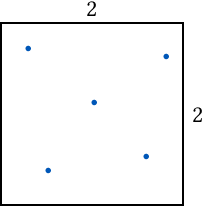
\includegraphics[width=\linewidth]{Images/image-2.png}}
\begin{proof}
    Divide square into 4 smaller squares. We now have 4 pigeonholes and 5 dots:
    \begin{figure}[H]
        \centering
        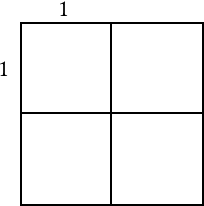
\includegraphics[width=100pt]{Images/image-3.png}
    \end{figure}
    These two points in the same pigeonhole have distance $\leq \sqrt{1^2+1^2}=\sqrt{2}$.
\end{proof}

\eg There exists two people in NYC who have exactly the same number of hairs on their head.

\eg There are 30 people at a party talking with each other. Afterwards, there will be two people who talked with the same number of people.
\begin{proof}
    If we put a person who talked to $i$ people into box $i$, we get 30 boxes; however, we cannot have someone who talked to 0 people and someone who talked at 29 people at the same time! Hence, we combine the box 0 and box 29, and only one of which could be the case.

    Now we have 29 boxes and 30 people. By pigeonhole principle, there must be two people who talked with the same amount of people.
\end{proof}

\begin{theorem}[Strong Pigeonhole Principle]
    Given pigeonholes $1,2,\dots,n$ with \uline{capacities} $c_1,c_2,\dots, c_n$ where $c_i\geq 0$; if we have at least $c_1+c_2+\dots+c_n+1$ pigeons in these pigeonholes, then at least one pigeonhole overflows.
\end{theorem}
\begin{proof}
    Suppose BWOC that no pigeonhole overflows. Then for all $i=1,2,\dots,n$, we have the number of pigeons in $i\leq c_i$.

    We add up and get inequalities:\begin{align*}
        \text{total \# pigeons} \leq c_1+c_2+\dots + c_n
    \end{align*}
    Contradiction!
\end{proof}

\eg There are five people supporting two teams. Then at least one team is supported by 3 people.
\begin{proof}
    Assume BWOC that the two teams only have two supporters. Let $c_1=c_2=2$. However, by SPP, $5\geq 2+2+1$, hence one pigeonhole overflows. Therefore, one team must have $>2$ supporters.
\end{proof}

\subsection{First Ramsey Theorem}

There are 6 people taking a class. Then: \begin{itemize}[align=left]
        \item[\underline{either}] there exists 3 people such that each pair of them have previously taken a class together,
        \item[\underline{or (inclusive)}] there exists 3 people such that no two have taken a class together.
    \end{itemize}

\begin{theorem}
    If we have 6 vertices and we draw all edges between them (a $K_6$ graph)\sidenote{$K_6$ stands for \textit{complete graph on 6 vertices.} It has 15 edges.}, then for every possible way of coloring the edges \rt{red} and \bt{blue}, there must exist a \textbf{monochromatic} triangle.

    \[\begin{tikzcd}[ampersand replacement=\&,cramped]
        \& \bullet \\
        \bullet \&\& \bullet \\
        \bullet \&\& \bullet \\
        \& \bullet
        \arrow[color=magenta, no head, from=1-2, to=2-1]
        \arrow[color=magenta, no head, from=1-2, to=2-3]
        \arrow[color=magenta, no head, from=2-3, to=3-3]
        \arrow[color=cyan, no head, from=3-3, to=4-2]
        \arrow[color=magenta, no head, from=4-2, to=3-1]
        \arrow[color=cyan, no head, from=2-1, to=2-3]
        \arrow[color=magenta, no head, from=2-3, to=3-1]
        \arrow[color=cyan, no head, from=3-1, to=2-1]
        \arrow[color=magenta, no head, from=2-1, to=3-3]
        \arrow[color=cyan, no head, from=3-3, to=3-1]
        \arrow[color=magenta, no head, from=1-2, to=4-2]
        \arrow[color=magenta, no head, from=2-1, to=4-2]
        \arrow[color=cyan, no head, from=4-2, to=2-3]
        \arrow[color=cyan, no head, from=1-2, to=3-3]
        \arrow[color=cyan, no head, from=1-2, to=3-1]
    \end{tikzcd}\]
\end{theorem}
\begin{proof}
    Pick any vertex and call it $A$. It has 5 edges colored \rt{red} and \bt{blue}. By the SPP, there exists at least 3 edges of the same color. WLOG let these three edges be \rt{red} and call the other three vertices $B,C,D$.
    \[\begin{tikzcd}[ampersand replacement=\&,cramped]
        \&\& {\bullet B} \\
        {A\,\bullet} \&\&\& {\bullet C} \\
        \&\& {\bullet D}
        \arrow[color=magenta, no head, from=2-1, to=1-3]
        \arrow[color=magenta, no head, from=2-1, to=2-4]
        \arrow[color=magenta, no head, from=2-1, to=3-3]
        \arrow[dashed, no head, from=1-3, to=2-4]
        \arrow[dashed, no head, from=3-3, to=2-4]
        \arrow[dashed, no head, from=1-3, to=3-3]
    \end{tikzcd}\]
    \begin{itemize}
        \item If $BC$ is \rt{red}, then $ABC$ is a \rt{red} triangle.
        \item If $CD$ is \rt{red}, then $ACD$ is a \rt{red} triangle.
        \item If $BD$ is \rt{red}, then $ABD$ is a \rt{red} triangle.
        \item If none of the above has happened, then $BC,CD,BD$ are all \bt{blue}, meaning that $BCD$ is a \bt{blue} triangle!
    \end{itemize}
\end{proof}

\begin{theorem}
    If there are 5 instead of 6 vertices, then the above coloring prediction cannot be made with certainty.
\end{theorem}
\begin{proof}[Counterexample]
    \[\begin{tikzcd}[ampersand replacement=\&,cramped,column sep=tiny]
        \&\& \bullet \\
        \bullet \&\&\&\& \bullet \\
        \& \bullet \&\& \bullet
        \arrow[color=magenta, no head, from=1-3, to=2-1]
        \arrow[color=cyan, no head, from=2-1, to=2-5]
        \arrow[color=magenta, no head, from=1-3, to=2-5]
        \arrow[color=cyan, no head, from=1-3, to=3-2]
        \arrow[color=cyan, no head, from=1-3, to=3-4]
        \arrow[color=magenta, no head, from=2-1, to=3-2]
        \arrow[color=magenta, no head, from=3-2, to=3-4]
        \arrow[color=magenta, no head, from=3-4, to=2-5]
        \arrow[color=cyan, no head, from=3-2, to=2-5]
        \arrow[color=cyan, no head, from=2-1, to=3-4]
    \end{tikzcd}\]
\end{proof}
\end{document} 
